\documentclass[a4paper,11pt]{book}
\usepackage{import}
\usepackage{preamb}

\makeindex

\begin{document}

\small
\begin{multicols}{3}

%\maketitle

\thispagestyle{empty}
\scriptsize
\newpage


\begin{subbox}{subbox}{}
\centering
\Large{\textbf{Network Science   \\ Cheatsheet}}
\end{subbox}

\begin{multibox}{2}
\begin{subbox}{subbox}{}
\centering

\includegraphics[width=0.8\textwidth]{pics/logo.png}
\end{subbox}
\begin{subbox}{subbox}{}
\centering
Made by \\
\large{
Remy Cazabet
}
\end{subbox}
\end{multibox}
% \section{Blocks and Community structure}


\begin{subbox}{subbox}{}
\centering
\Large{\textbf{Graph/Node embedding}}
\end{subbox}


\begin{subbox}{subbox}{Disclaimer}
Graph/Node embeddings are a recent field of research, with hundreds of publications in the last few years, and scores of new papers published in every machine learning and network science conference. This class is thus only an introduction to the mechanism underlying those approaches.
\end{subbox}


\begin{textbox}{Embedding of networks}
In the context of \textbf{graph embedding}, embedding is a shortcut for \textbf{embedding in low dimensions}, and can be understood as assigning to some \textbf{elements} of the graph a \textbf{vector} (i.e., a list of numbers) composed of \textbf{d} elements. \textbf{d} is the number of dimensions in the embedding space, and \textbf{d} should be small.
\end{textbox}

\begin{textbox}{Types of Network Embedding}
According to the type of element which is embedded, we can differentiate:
\begin{itemize}
    \item Node Embedding (one vector per node)
    \item Edge Embedding (one vector per edge)
    \item Substructure Embedding (e.g., one vector per community)
    \item Whole Graph Embedding (one vector per graph)
\end{itemize}

In this class, we will introduce only Node Embedding, which is the most popular approach.

Whole graph embedding is also quite popular, for instance to classify types of networks.
\end{textbox}


\begin{textbox}{Node Embedding}
In \textbf{node embedding}, the vector assigned to each node should be a proxy, a sort of numeric summary of the position of the node in the graph, in term of topology. Several types of embeddings exist that capture different aspects of the network topology, in particular we will differentiate \textit{locational embedding} from \textit{role embedding}. Note that node embedding is sometimes called \textbf{graph embedding} in the literature.
\end{textbox}

\begin{textbox}{Embedding distance}
Since each node is represented by a vector, it is possible to compute a \textbf{distance between nodes} in the embedding. Intuitively, two nodes occupying similar positions in the network (according to what the chosen embedding capture) should have similar embedding vectors. The notion of distance to use (cosine, euclidean, etc.) also depends on the chosen embedding.
\end{textbox}

\begin{textbox}{Adjacency matrix(A) as an embedding}
A naive way to choose an embedding (in $n$ dimensions) could be to consider each row of the adjacency matrix as the vector representation of the node it corresponds to. 

This embedding would capture what is called the \textbf{structural equivalence}, i.e. the fact that nodes share similar neighborhoods. Two nodes with the same neighborhoods would have the same vectors. If the \textit{Manhattan distance} were used, the distance between nodes in the embedding would correspond to the number of different neighbors.
\end{textbox}

\begin{textbox}{What is a good embedding?}
What is a good embedding depends on the task that we want to achieve. In the perspective of this class, embeddings are mostly used as features for machine learning tasks. As such, they must be 1) In as few dimensions as possible: Machine learning suffers from what is known as the \textbf{curse of dimensionality}, and tends to work better with lower dimensions, without talking about computational advantages. 2) As dense as possible. Sparsity --usually associated with high dimensions-- makes learning harder.

Furthermore, the embedded properties must be meaningful for the task to achieve. For instance, the notion of distance captured by the adjacency matrix seems in contradiction with the intuition: in graphs, one usually use the number of common neighbors, and/or normalized fraction of neighbors (Jaccard, etc.) rather than a raw count of different neighbors.
\end{textbox}


\begin{textbox}{Embedding and Dimensionality Reduction}
In Machine Learning, when a dataset is composed of too many features, \textbf{dimensionality reduction} algorithms can be used to generate a smaller number of synthetic features, defined as combination of the original ones. Common algorithms to do so are for instance \textbf{PCA} (Principal Component Analysis) and \textbf{T-SNE}\footcite{maaten2008visualizing}. 

A simple method to generate a better embedding from the adjacency matrix would be to apply Dimensionality Reduction on it to reduce its number of dimension. Its counter-intuitive definition of distance would nevertheless remain a problem. 
\end{textbox}



\begin{textbox}{Notations}
\begin{tabular}{p{0.12\textwidth}|p{0.8\textwidth}}\scriptsize
$y$ & Embedding of the graph \\
$y_i$ & Vector corresponding to node $i$ in the embedding $y$\\
$S$ & Similarity matrix. For each pair of node $i,j$, $S_{ij}$ represents the graph similarity that we want to preserve. 
\end{tabular}
By default, $S=A$: two nodes have a maximal similarity of 1 if they are connected, and similarity 0 if they are not connected. But one can use a different notion, such as a random walk distance, a neighborhood similarity heuristic, etc. 
\end{textbox}


\begin{textbox}{Node Embedding: LE}
\textbf{Laplacian Eigenmaps} (LE)\footnote{Belkin2003LaplacianEF} is a method that can be used for node embedding, whose objective function is defined as follows:
\[
y=\min \sum_{i\neq j}\lVert y_i - y_j \rVert ^2 S_{ij}
\]
This can be read as follows: to find the embedding $y$ of a graph, we need to assign an embedding $y_i$ to each node $i$ such as the sum (over all node pairs) of the equation $\lVert y_i - y_j \rVert ^2 S_{ij}$ is minimal.
Said differently, its objective is to minimize the product between the \textbf{euclidean distance} in the embedding ($\lVert y_i - y_j \rVert ^2$) and the \textbf{similarity} in the graph $S_{ij}$.

If two nodes are similar/close in the graph (high value), we need to make them as close as possible in the embedding (small value). Nodes dissimilar/distant in the graph can be distant in the embedding with a lesser penalty. To forbid a trivial solution of all nodes being on the same location, the sum of distance between points in the embedding must be equal to a constant.
\end{textbox}



\begin{textbox}{Node Embedding: HOPE}
\textbf{Higher-Order Proximity preserved Embedding}  (HOPE)\footnote{ou2016asymmetric} objective function is:
\[
y=\min \sum_{i,j} |S_{ij}-y_i y_j^T |
\]
Said differently, its objective is to minimize the difference between the graph \textbf{similarity} $S_{ij}$ and the similarity in the embedding, computed as the product of embedding vectors. Vectors are imposed to be normalized, thus $y_i y_j^T$ corresponds to the \textit{cosine similarity}.

Two nodes close (resp. far) in the graph should therefore be close (far) in the embedding. Relative distances should also be conserved.
\end{textbox}


\begin{textbox}{LE - HOPE: Complexity}
Discovering the solution of LE and HOPE methods can be done efficiently using matrix decomposition approaches. For instance, finding the embedding according to LE in $d$ dimensions for the adjacency matrix can be formalized as finding the $d$ eigenvectors of lowest eigenvalues of $D^{-1/2}LD^{-1/2}$, with $D$ the degree matrix and $L$ the Laplacian matrix.

The computation of the $S$ matrix however, if it is not the adjacency matrix, can be costly since in the general case, it requires $n^2$ computations.
\end{textbox}



\begin{textbox}{Random Walk NN based embedding}
In recent years, new approaches based on random walks and neural networks have encountered a large success and relaunched a large interest in graph embedding for various applications. They are transpositions of techniques developed for the embedding of words to the graph setting.
\end{textbox}

\begin{textbox}{Word Embedding}
Machine Learning on text suffers from a problem similar to Machine Learning on graphs: words are not numbers and cannot be naturally represented as (meaningful) vectors. Word embedding objective is to assign a (low dimensional) vector to each word such as two words with \textbf{similar semantic} have similar vectors.
\end{textbox}

\begin{subbox}{subbox}{Matrix decomposition and Eigenvectors}
A diagonizable matrix $A$ can be factorized using eigenvectors as follows:
\[
\mathbf{A}=\mathbf{Q}\mathbf{\Lambda}\mathbf{Q}^{-1}  
\]
where $Q$ is the  $n \times n$ matrix whose $i$th column is the eigenvector $q_i$ of $A$, and $\mathbf{\Lambda}$ is the diagonal matrix whose diagonal elements are the corresponding eigenvalues, $\mathbf{\Lambda}_{ii} = \mathbf{\lambda}_i$. Keeping as embedding the eigenvectors associated with the largest eigenvalues means that we can reconstruct the original matrix with a good precision. This is the same method used by PCA (Principal Component Analysis), on a covariance(or correlation) matrix, which is also a form of similarity matrix.
\end{subbox}

\begin{textbox}{Word Embedding: word2vec - context}
The principle proposed in a famous method called word2vec is to use the context, i.e., the words encountered around a word in sentences of a corpus, to discover the semantic similarity. In summary, the more two words are encountered in a same context, the more they are considered similar. For instance, a corpus might contain sentences such as: \textit{the dog eat dry food}, and \textit{the cat eat dry food}: \textit{cat} and \textit{dog} are found in similar contexts, which should drive them closer in the embeddding. In other sentences, their contexts differs, which should drive them away in the embedding.
\end{textbox}

\begin{textbox}{Word Embedding: Skipgram/word2vec}
In practice, a word is considered to be in the context of another if it is at a distance less than $l$ in a sentence. From a corpus, one then extracts the probability $p(w_j|w_i)$ for each word $w_i$, that a word taken at random in its context is $w_j$.

The objective function of word2vec can be expressed as:
\[
y=\min \sum_{(i,j)} p(w_j|w_i)-\sigma(y_i y_j^T)
\]
with $\sigma$ the softmax function defined as $\frac{e^x}{\sum e^x}$, a function commonly used in neural networks to add non-linearity while ensuring that the solution is a probability.
\end{textbox}


\begin{textbox}{Skipgram: a neural network formulation}
The skipgram algorithm is solved, in practice, using tools and methods of neural networks, which make it scalable to large datasets. It can then be represented as follows:

\centering

\colorbox{white}{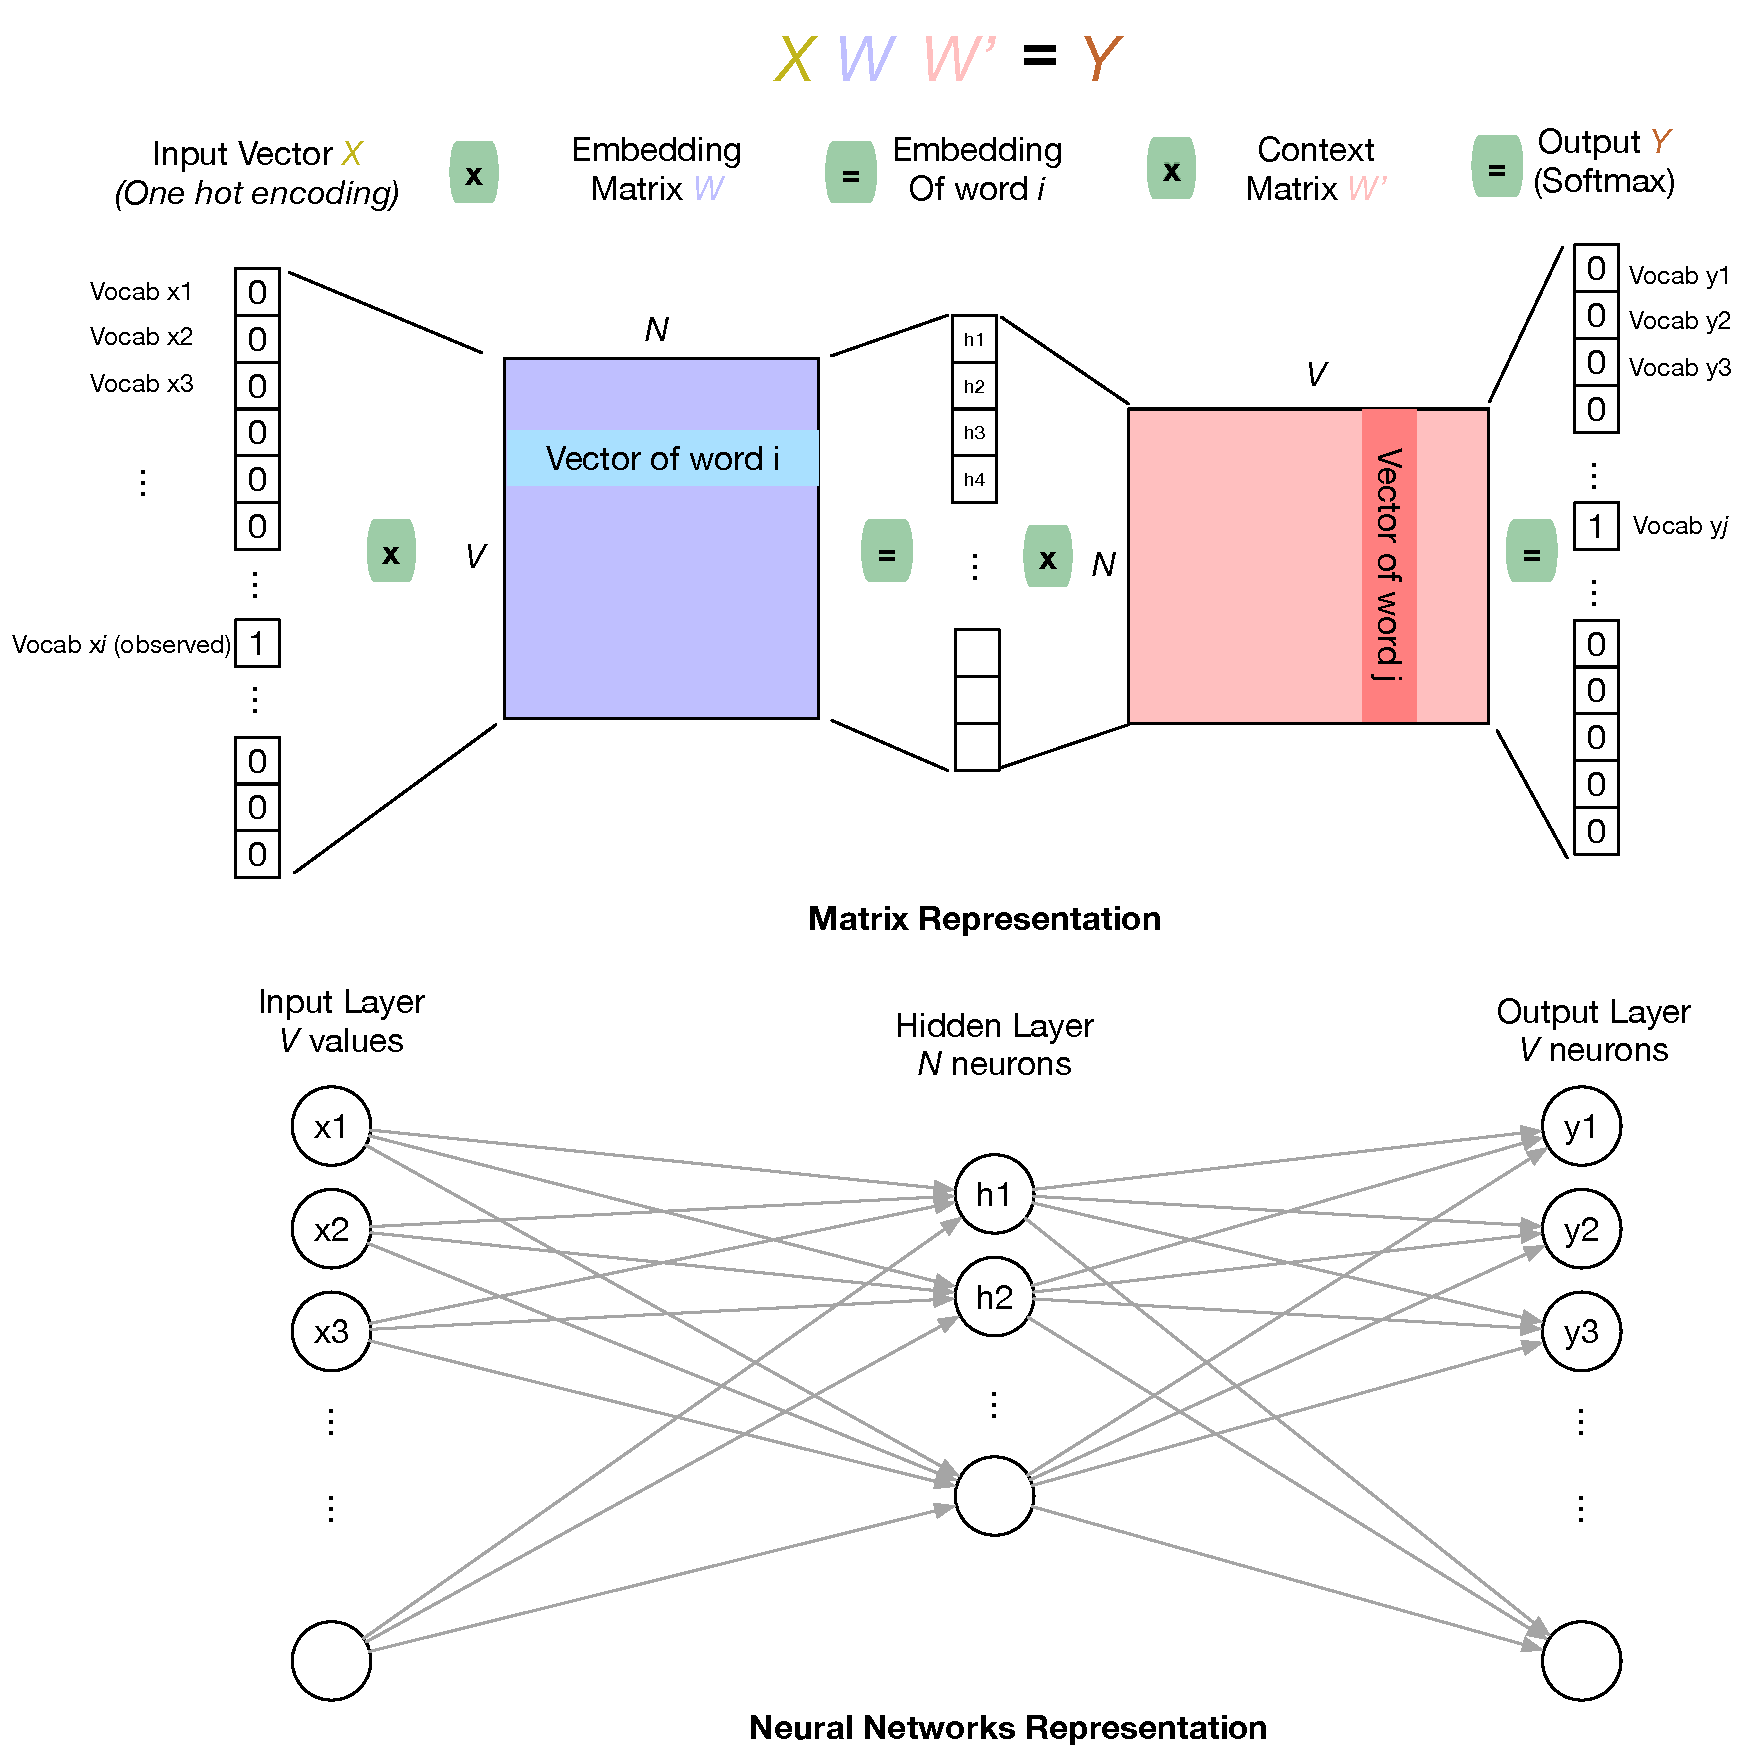
\includegraphics[width=0.8\linewidth]{pics/skipgram.pdf}}
\end{textbox}


\begin{textbox}{Word2vec efficacy}
Word2Vec (and following word embedding approaches) have encountered an enormous success in the Natural Language Processing domain, and its descendants are used for most practical tasks such as automatic language translation, sentiment analysis, personal assistants, etc.

Various other fields, including network science, have therefore adapted the mechanism to embed other complex items.
\end{textbox}


\begin{textbox}{DeepWalk}
DeepWalk\footcite{perozzi2014deepwalk} is the direct transcription of Word2vec to graphs. The principle is to generate random walks in the graph, playing the role of sentences in a corpus. The probability of finding a word in the vicinity of another therefore translates in the probability of encountering a node in the context window of another, i.e., at a short random-walk distance.

To sum up, the objective function can now be expressed as:
\[
y=\min \sum_{(i,j)} p(n_j|n_i)-\sigma(y_i y_j^T)
\]
with $p(n_j|n_i)$ the probability to encounter node $n_j$ in the context of node $n_i$. Its objective is therefore to make the distance in the embedding proportional to a random walk based distance in the graph.
\end{textbox}

\begin{textbox}{DeepWalk complexity}
Contrary to matrix decomposition based approaches, DeepWalk do not requires explicitly a similarity matrix $S$. All pairs $(i,j)$ are obtain by $k$ random walks of length $l$ starting from each of the $n$ nodes. The complexity of obtaining the input data is therefore in $\mathcal{O}(n)$ ($l$ and $k$ being small constants).
\end{textbox}

\begin{textbox}{Node2vec}
\textbf{Node2vec}\footcite{grover2016node2vec} is a popular variant of DeepWalk, introducing \textbf{biased random walks}. Two parameters guide the random walks: $p$ affect the probability to revisit the previous node, while $q$ affect the probability to explore farther nodes, i.e., nodes that were not neighbors of the origin node. It allows to mimic \textbf{breadth-first} or \textbf{depth-first} like exploration of the graph, capturing more local or more global network structures.
\end{textbox}

\begin{textbox}{Node2vec}
Illustration of random walk procedure in node2vec. 

\centering
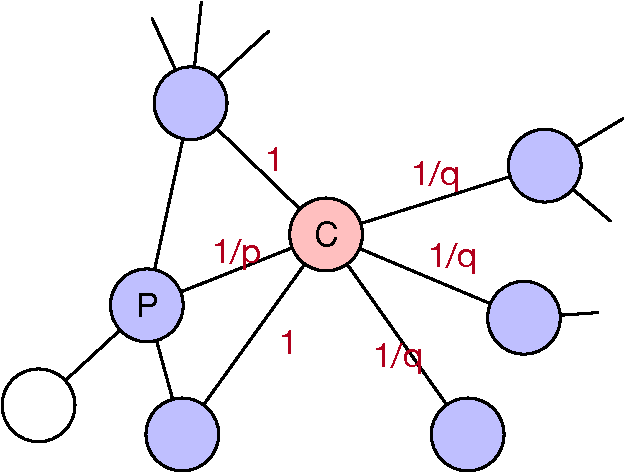
\includegraphics[width=0.6\linewidth]{pics/n2v.pdf}


The walk just transitioned from the previous node $p$ to the current one $c$ and is now evaluating its next hop. Edge labels indicate the bias as a function of parameters $p$ and $q$.
\end{textbox}



\begin{textbox}{Role Embedding}
Node2Vec and DeepWalk are \textbf{locational} embedding: nodes with similar vectors tend to be close in the graph, in term of graph distance.

Another notion of graph similarity is \textbf{role} similarity. Two nodes have similar roles in the graph if their neighborhood is similar, \textbf{ignoring node labels}. 
\end{textbox}



\begin{textbox}{Role2Vec — Struc2Vec}
Two popular methods for role embedding are Struc2Vec\footcite{ribeiro2017struc2vec} and Role2Vec\footcite{ahmed2019role2vec}. They are based on a similar principle: as DeepWalk, they use random walks and SkipGram to generate embedding from contexts. But instead of generating sequences composed of the \textbf{labels} of encountered nodes, it generate contexts based on the \textbf{attributes/labels/features} of encountered nodes. Nodes with similar vectors thus corresponds to nodes that tend to encounter \textbf{nodes with similar properties} in random walks starting from them.

Examples of properties could be node features (age, genre, etc.) or structural properties (degree, clustering coefficient, graphlet belonging, etc).
\end{textbox}



\begin{textbox}{Node Classification with embeddings}
Machine Learning algorithms such as Logistic Regression or Decision Tree can be trained to predict a property of a node from a vector of features representing the node property. We have seen in a previous class that these features could be manually chosen heuristics such as node centralities. 

Vectors yielded by embedding algorithms can naturally be used in the same way. Locational embeddings could be used, for instance to attribute category to objects or political opinions to social media accounts, while role embedding could be used to identify suspicious accounts in social media.
\end{textbox}



\begin{textbox}{Link Prediction with embeddings: unsupervised}
If we consider that the property captured by the embedding is correlated with the probability of being connected by an edge, then the distance in the embedding can be used a heuristic for link prediction. 

For instance, with LE and HOPE with $S=A$ or with random walks based approach, the embedding tries to put pairs of nodes connected by an edge closer than unconnected ones. As a consequence, we can assume that the closer two nodes are in the embedding, the more likely it is that they should be connected by an edge.
\end{textbox}



\begin{textbox}{Link Prediction with embeddings: supervised}
In the second approach, we consider each dimension of the embedding as a node feature. For each pair of nodes, we compute a vector by \textbf{combining nodes' vectors}.

As with heuristics, a machine learning algorithm is then trained to predict, from the combined vector, how likely it is to have an edge between nodes.
\end{textbox}




\begin{textbox}{Combining node vectors}
There are several methods to combine node vectors. Although it has been observed empirically that the Hadamard product often gives the best results, this choice is often considered a \textbf{hyper-parameter}, i.e., all variants are tested and the most efficient is used for the final prediction.

The most used operators are:
\begin{center}
\begin{tabular}{ c| c }
\hline
 Average & (a+b)/2 \\ 
 \hline
 Concat & $[a_1,a_2,...,a_d,b_1,b_2,...,b_d]$\\  
 Hadamard & $[a_1*b_1,a_2*b_2,...,a_d*b_d]$  \\
  Weighted L1 & $[|a_1-b_1|,|a_2-b_2|,...,|a_d-b_d|]$ \\ 
 Weighted L2 & $[(a_1-b_1)^2,(a_2-b_2)^2,...,(a_d-b_d)^2]$\\  
 \hline
\end{tabular}

with $a=[a_1,a_2,...,a_d]$ and $b=[b_1,b_2,...,b_d]$
\end{center}
\end{textbox}


\begin{textbox}{How many dimensions?}
There is no universal method to choose a number of dimensions for the embedding. In the literature, for large graphs, a common value is $d=128$ dimensions. As a general rule, $d<<n$.

Too few dimensions limit the capacity to embed complex information, but too many dimensions limit cross-learning, generalization,(i.e., overfits), and make learning from embeddings harder. More dimensions also require (usually) more computation.
\end{textbox}

\begin{textbox}{Visualization and embeddings}
Network visualization is a domain in itself. Its objective is to assign positions to nodes in a two dimensional space in order to plot the network in a meaningful way. 

Algorithms such as HOPE or node2vec are not well adapted to generate visually interpretable 2-dimentional spaces, in part because the distance in the embedding is based on the cosine distance, while humans naturally assume euclidean distance. When embeddings are used for visualization, the first step consists in embedding in a moderate number of dimensions (e.g., 128), and in a second step, a dimensionality reduction algorithm more adapted for visualization such as T-SNE\footcite{van2008visualizing} is used to reduce this number to 2 dimensions.
\end{textbox}


\begin{textbox}{Community detection with embeddings}
Community detection in graphs is equivalent to the \textbf{clustering} task in non-network data. Intuitively, clustering methods try to group elements with similar features, and separate those that are different. Applying a clustering algorithm such as \textbf{k-means} on an embedding will therefore yield clusters of nodes, that can be considered as communities. In practice, it has been observed that communities detected by this approach are often similar to those found by modularity maximization.

Note that unlike with modularity, it is often required to provide the desired number of clusters --or a distance scale-- to clustering methods.
\end{textbox}

\begin{textbox}{Going Further}

Python Libraries: Karate-club(\cite{karateclub})(\cite{goyal2018gem})

Surveys on graph embedding: (\cite{goyal2018graph})(\cite{cai2018comprehensive})(\cite{cui2018survey})

Graph Embedding and link prediction (\cite{mara2020benchmarking})

Distances in Graph embedding (\cite{vaudaine2020comparing})

Comparing heuristics and Graph Embedding for link prediction (\cite{sinha2018systematic})

Stacking embeddings and heuristics models for link prediction: (\cite{ghasemian2020stacking})

\end{textbox}


 \AtNextBibliography{\footnotesize}


\printbibliography[heading=subbibliography]


\end{multicols}







\end{document}


